\documentclass[11pt,letterpaper]{article}
\PassOptionsToPackage{hyphens}{url}
\usepackage[margin=.83in,top=.8in,bottom=.8in,headheight=15pt]{geometry}
\usepackage[T1]{fontenc}
\usepackage{lmodern,amsmath,amssymb,mathtools,bm,booktabs,array,graphicx,tikz}
\usetikzlibrary{arrows.meta,positioning,calc,decorations.pathreplacing,patterns}
\definecolor{ink}{HTML}{17344D}\definecolor{accent}{HTML}{087E8B}\definecolor{pale}{HTML}{EDF5F5}\definecolor{gold}{HTML}{AD6B19}
\providecommand{\dd}{\,\mathrm{d}}\providecommand{\R}{\mathbb{R}}
\providecommand{\E}{\mathbb{E}}\providecommand{\Var}{\operatorname{Var}}
\providecommand{\Cov}{\operatorname{Cov}}\providecommand{\diag}{\operatorname{diag}}
\providecommand{\norm}[1]{\left\lVert#1\right\rVert}
\providecommand{\abs}[1]{\left|#1\right|}
\usepackage{microtype,hyperref,fancyhdr,enumitem,amsthm,sectsty,needspace}
\allsectionsfont{\raggedright}
\hypersetup{colorlinks=true,linkcolor=ink,urlcolor=accent,pdfauthor={Zan Ahmad},pdftitle={Resistance, compliance, and the reservoir equation / Lecture notes}}
\setlength{\parindent}{0pt}\setlength{\parskip}{6pt}\linespread{1.07}
\setlist{itemsep=3pt,topsep=4pt,leftmargin=*}
\emergencystretch=2em\clubpenalty=10000\widowpenalty=10000
\pagestyle{fancy}\fancyhf{}\fancyhead[L]{\small Mathematical Cardiology}\fancyhead[R]{\small Lecture 2}
\fancyfoot[L]{\footnotesize Zan Ahmad}\fancyfoot[R]{\footnotesize\thepage}\renewcommand{\headrulewidth}{.3pt}
\newtheorem{proposition}{Proposition}\newtheorem{theorem}{Theorem}\newtheorem{lemma}{Lemma}
\theoremstyle{definition}\newtheorem{definition}{Definition}\newtheorem{example}{Example}
\numberwithin{equation}{section}
\begin{document}
{\small\scshape Mathematical Cardiology\hfill Lecture 2}\par\medskip
{\raggedright\hyphenpenalty=10000\exhyphenpenalty=10000\LARGE\bfseries\color{ink} Resistance, compliance, and the reservoir equation\par}\medskip
{\small Lecture notes}\par\bigskip
A vessel can transmit blood and store blood. These are different operations, governed by different pressure differences. We shall describe each separately and then combine them with conservation. The resulting reservoir is the first time-dependent model in the course: a pressure changes because inflow and outflow do not initially balance.

\section{Two pressure differences and two constitutive laws}
\hypertarget{note-two-pressure-differences-and-two-constitutive-laws}{}\label{note:two-pressure-differences-and-two-constitutive-laws}
{\small \href{slides.html\#frame=transmission-and-storage\&step=1}{Slides for this section}}\par
The pressure drop along a connection is $P_{\rm in}-P_{\rm out}$. The pressure across a vessel wall is the transmural pressure $P_{\rm tm}=P-P_{\rm ext}$. A vessel can have the same pressure at both ends and still be distended, because its internal pressure can exceed its external pressure.

For a passive resistance and a linear elastic reservoir, respectively, write
\begin{equation}
Q=\frac{P_{\rm in}-P_{\rm out}}{R},\qquad
V=V_d+C(P-P_{\rm ext}).
\end{equation}
Here $R>0$ and $C>0$. In this lesson, $Q$ is in mL/s, $R$ in $\mathrm{mmHg\,s/mL}$, and $C$ in $\mathrm{mL/mmHg}$. Compliance is not the reciprocal of resistance: $1/R$ has units of flow per pressure, whereas $C$ has units of volume per pressure. Their product has units of time.

The constant $V_d$ is a reference volume. It prevents the linear approximation from asserting that zero transmural pressure necessarily means zero vessel volume. The approximation need not remain valid near collapse or at large distension. Real walls can have nonlinear pressure--volume relations, and resistance can change with geometry and smooth-muscle activity.

For constant $C$ and fixed external pressure, subtraction at two times gives $\Delta V=C\Delta P$. This is the relation needed for changes. If external pressure also changes, it is $C\Delta(P-P_{\rm ext})$ that appears instead.
\section{Combine storage with a volume balance}
\hypertarget{note-combine-storage-with-a-volume-balance}{}\label{note:combine-storage-with-a-volume-balance}
{\small \href{slides.html\#frame=a-reservoir-with-a-prescribed-supply\&step=1}{Slides for this section}}\par
Supply a reservoir at a constant inflow $I$, and drain it through resistance $R$ into an outlet held at pressure $P_o$. The reservoir pressure is $P(t)$. Its outflow is $(P-P_o)/R$; the inflow is an independently prescribed input, not a second resistance law.

Choose times $t_n=n h$, with $h$ in seconds. Evaluate outflow at the start of each interval and approximate the volume change by that starting net flow:
\begin{align}
V_{n+1}-V_n&\approx h\left(I-\frac{P_n-P_o}{R}\right),\\
C(P_{n+1}-P_n)&\approx h\left(I-\frac{P_n-P_o}{R}\right).
\end{align}
This gives the explicit update
\begin{equation}
P_{n+1}=P_n+\frac hC\left(I-\frac{P_n-P_o}{R}\right).
\end{equation}
The update is exact for its chosen piecewise-constant approximation, not generally for the changing physical flow. A shorter interval reduces the amount of within-step change that we ignore.

With $I=2$ mL/s, $P_o=P_0=5$ mmHg, $R=10\ \mathrm{mmHg\,s/mL}$ and $C=2$ mL/mmHg, the first outflow is zero. For $h=1$ s, the update stores approximately $2$ mL and raises pressure by $1$ mmHg. On the next step, outflow is already positive; continuing to add $1$ mmHg every second would ignore the feedback through the outlet.
\section{Equilibrium and the error recurrence}
\hypertarget{note-equilibrium-and-the-error-recurrence}{}\label{note:equilibrium-and-the-error-recurrence}
{\small \href{slides.html\#frame=equilibrium-is-a-flow-balance\&step=1}{Slides for this section}}\par
At equilibrium there is no accumulation, so outflow equals inflow:
\[
I=\frac{P_\infty-P_o}{R},\qquad P_\infty=P_o+RI.
\]
The example therefore approaches $25$ mmHg. Compliance does not appear in this equilibrium formula because, once storage stops changing, the required pressure drop is determined by resistance and flow.

Subtract $P_\infty$ from the update and define $e_n=P_n-P_\infty$. Since $I=(P_\infty-P_o)/R$,
\begin{align}
e_{n+1}&=e_n-\frac h{RC}e_n
=\left(1-\frac h{RC}\right)e_n,\\
e_n&=\left(1-\frac h{RC}\right)^n e_0.
\end{align}
Thus $RC$ is a time scale. Here it is $20$ seconds. For $0<h/(RC)\leq1$, each new pressure lies between the old pressure and the equilibrium; the numerical approach does not overshoot. For $1<h/(RC)<2$, the recurrence still converges but alternates about equilibrium. At or beyond the remaining stability boundary it need not converge. A poor step size can therefore introduce behavior that is absent from the continuous reservoir.
\section{The exponential response}
\hypertarget{note-the-exponential-response}{}\label{note:the-exponential-response}
{\small \href{slides.html\#frame=the-continuous-balance\&step=1}{Slides for this section}}\par
The short-step balance has a continuous-time notation,
\begin{equation}
C\frac{dP}{dt}=I-\frac{P-P_o}{R}.
\end{equation}
The derivative means the instantaneous rate of pressure change. Students who have not studied calculus can read this as the limiting version of the finite-step accounting. Writing $e=P-P_\infty$ reduces it to $de/dt=-e/(RC)$. The solution is
\begin{equation}
P(t)=P_\infty+(P_0-P_\infty)e^{-t/(RC)}.
\end{equation}
This formula can also be motivated by the recurrence: over a fixed duration, repeatedly retaining a factor $1-h/(RC)$ tends toward exponential retention as $h$ decreases.

At $t=0$, the exponential equals one and returns $P_0$. At long times it tends to zero and returns $P_\infty$. After one time constant, the remaining distance to equilibrium is $e^{-1}\approx0.368$ of its starting value. For the example, $P(1)=25-20e^{-1/20}\approx5.9754$ mmHg, slightly below the initial-rate estimate of $6$ mmHg.

Increasing $C$ changes the time constant without changing the final pressure when $I,R,P_o$ remain fixed. This is the reason the three supplied curves approach the same level at different speeds. It also separates two measurements: the final pressure can identify $R=(P_\infty-P_o)/I$ when $I\ne0$, while a time constant can then identify $C=\tau/R$. One final pressure alone cannot identify compliance.
\begin{center}\begin{minipage}{.98\linewidth}\centering
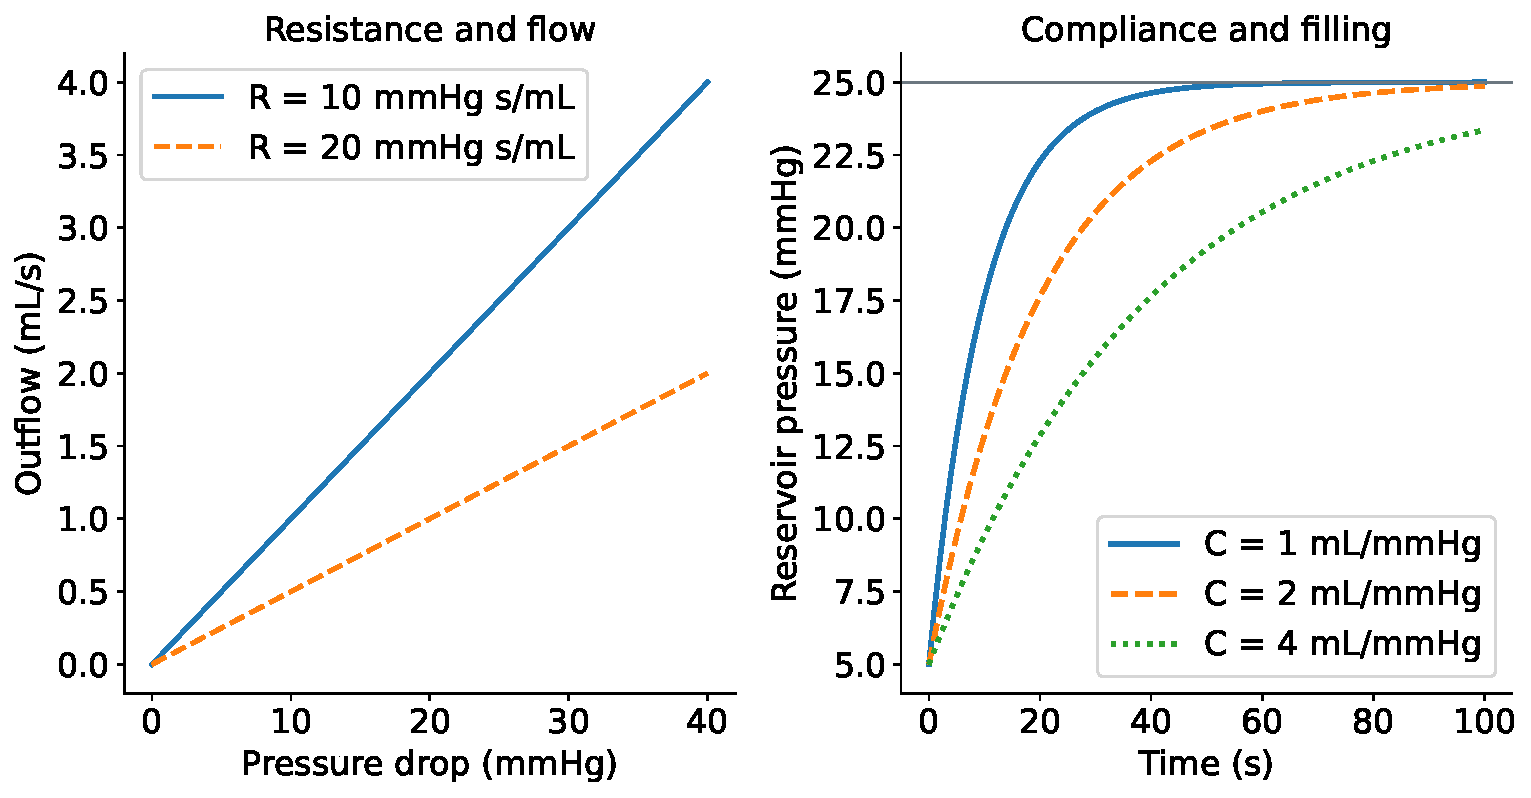
\includegraphics[width=.96\linewidth,height=.57\textheight,keepaspectratio]{pressure-storage.pdf}\par\smallskip
{\small Synthetic reservoir: inflow 2 mL/s, outlet and starting pressure 5 mmHg, resistance 10 mmHg s/mL. Changing compliance changes approach speed but not the 25 mmHg final pressure.}
\end{minipage}\end{center}
\section{Spatial resolution and the question being asked}
\hypertarget{note-spatial-resolution-and-the-question-being-asked}{}\label{note:spatial-resolution-and-the-question-being-asked}
{\small \href{slides.html\#frame=two-measurements-for-two-parameters\&step=1}{Slides for this section}}\par
A compartment model assigns one pressure and one volume to a whole region. This is called a zero-dimensional model because it does not resolve positions within that region, not because the region lacks physical size. Its balance can be useful for stored volume or average pressure, but it cannot locate a jet or a wall-stress concentration.

A one-dimensional vessel model retains distance along a vessel. Its area and average flow depend on position and time, allowing a description of pulse propagation when appropriate fluid and wall laws are supplied. The speed of a pressure disturbance is not automatically the speed of an individual blood cell. A three-dimensional model resolves a local velocity field and geometry, requiring more boundary information and numerical resolution.

These descriptions answer different questions. Adding spatial detail does not supply missing inflow data or make uncertain material parameters known. A reservoir calculation can be checked by its equilibrium, its units, its initial slope and its short-step limit. To validate it as a description of an actual vessel requires independent pressure and volume observations. For a project, measurements that distinguish $R$ from $C$ are more informative than a visually elaborate curve whose parameters cannot be separated.
\begin{center}\begin{minipage}{.98\linewidth}\centering
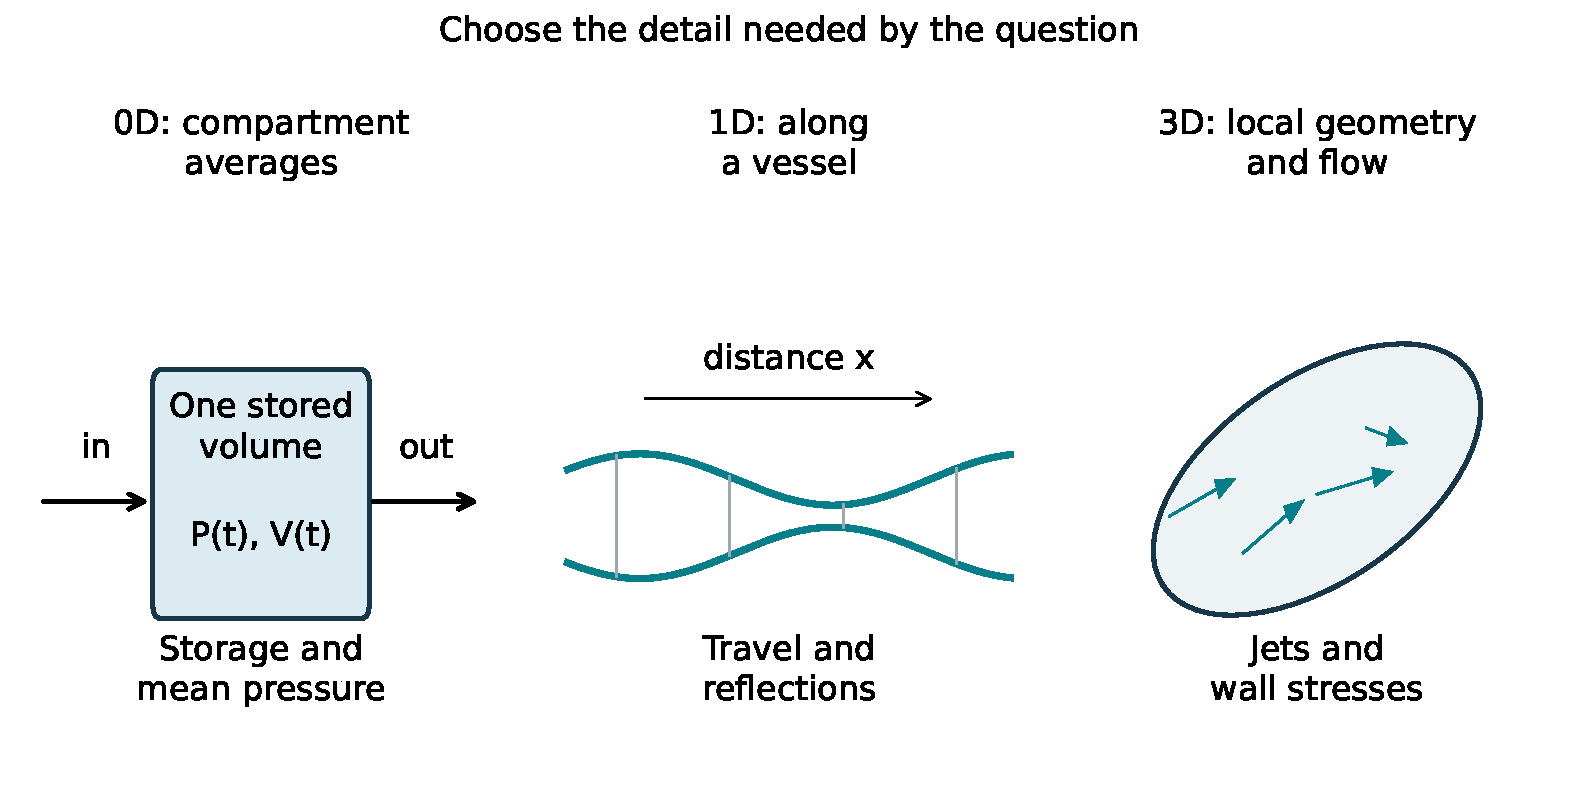
\includegraphics[width=.96\linewidth,height=.57\textheight,keepaspectratio]{presentation-figures/model-scales.pdf}\par\smallskip
{\small Original schematics distinguish compartment averages, variation along a vessel, and a local 3D flow region. They are not computed flow solutions.}
\end{minipage}\end{center}
\bigskip
\section*{Exercises}
\par\noindent\begin{minipage}{\linewidth}
\subsection*{MC02-E1. Keep the units with the numbers}
Use a passive resistor with resistance 8 mmHg s/mL, inlet 29 mmHg and outlet 5 mmHg.

\textbf{a} Find the flow and show its unit cancellation.

\end{minipage}\par\medskip
\textbf{b} Add 12 mmHg to both pressures. What changes?

\textbf{c} Double resistance with the original pressures. State an assumption and a limitation.

\par\noindent\begin{minipage}{\linewidth}
\subsection*{MC02-E2. Account for stored volume}
During one specified two-second interval, inflow and outflow are constant at 4 and 1 mL/s. Compliance is 3 mL/mmHg and external pressure is fixed.

\textbf{a} Find the change in stored volume.

\end{minipage}\par\medskip
\textbf{b} Find the change in pressure.

\textbf{c} If compliance doubles, compare the volume and pressure changes. Explain why this is not a steady-state calculation.

\par\noindent\begin{minipage}{\linewidth}
\subsection*{MC02-E3. Select a model and evidence}
A team wants to study average arterial storage, pulse arrival along an artery, and a jet beside a valve.

\textbf{a} Match each question to the simplest suitable 0D, 1D or 3D description.

\end{minipage}\par\medskip
\textbf{b} Name one input and one validation observation for the pulse-arrival question.

\textbf{c} Draft a narrow project question and state one limitation that a more detailed picture alone would not remove.

\section*{References}
\noindent\begin{minipage}{\linewidth}
Zan Ahmad, Fall 2023 HEART syllabus. Public PDF pp. 1--2, Course Topics and Course Expectations; editable syllabus pp. 2--3, project requirements.

\end{minipage}\par\medskip
\noindent\begin{minipage}{\linewidth}
Hoppensteadt and Peskin, Modeling and Simulation in Medicine and the Life Sciences, second edition. Printed pp. 8--10; PDF pp. 21--23, section 1.3.

\end{minipage}\par\medskip
\end{document}
